\documentclass[1p]{elsarticle_modified}
%\bibliographystyle{elsarticle-num}

%\usepackage[colorlinks]{hyperref}
%\usepackage{abbrmath_seonhwa} %\Abb, \Ascr, \Acal ,\Abf, \Afrak
\usepackage{amsfonts}
\usepackage{amssymb}
\usepackage{amsmath}
\usepackage{amsthm}
\usepackage{scalefnt}
\usepackage{amsbsy}
\usepackage{kotex}
\usepackage{caption}
\usepackage{subfig}
\usepackage{color}
\usepackage{graphicx}
\usepackage{xcolor} %% white, black, red, green, blue, cyan, magenta, yellow
\usepackage{float}
\usepackage{setspace}
\usepackage{hyperref}

\usepackage{tikz}
\usetikzlibrary{arrows}

\usepackage{multirow}
\usepackage{array} % fixed length table
\usepackage{hhline}

%%%%%%%%%%%%%%%%%%%%%
\makeatletter
\renewcommand*\env@matrix[1][\arraystretch]{%
	\edef\arraystretch{#1}%
	\hskip -\arraycolsep
	\let\@ifnextchar\new@ifnextchar
	\array{*\c@MaxMatrixCols c}}
\makeatother %https://tex.stackexchange.com/questions/14071/how-can-i-increase-the-line-spacing-in-a-matrix
%%%%%%%%%%%%%%%

\usepackage[normalem]{ulem}

\newcommand{\msout}[1]{\ifmmode\text{\sout{\ensuremath{#1}}}\else\sout{#1}\fi}
%SOURCE: \msout is \stkout macro in https://tex.stackexchange.com/questions/20609/strikeout-in-math-mode

\newcommand{\cancel}[1]{
	\ifmmode
	{\color{red}\msout{#1}}
	\else
	{\color{red}\sout{#1}}
	\fi
}

\newcommand{\add}[1]{
	{\color{blue}\uwave{#1}}
}

\newcommand{\replace}[2]{
	\ifmmode
	{\color{red}\msout{#1}}{\color{blue}\uwave{#2}}
	\else
	{\color{red}\sout{#1}}{\color{blue}\uwave{#2}}
	\fi
}

\newcommand{\Sol}{\mathcal{S}} %segment
\newcommand{\D}{D} %diagram
\newcommand{\A}{\mathcal{A}} %arc


%%%%%%%%%%%%%%%%%%%%%%%%%%%%%5 test

\def\sl{\operatorname{\textup{SL}}(2,\Cbb)}
\def\psl{\operatorname{\textup{PSL}}(2,\Cbb)}
\def\quan{\mkern 1mu \triangleright \mkern 1mu}

\theoremstyle{definition}
\newtheorem{thm}{Theorem}[section]
\newtheorem{prop}[thm]{Proposition}
\newtheorem{lem}[thm]{Lemma}
\newtheorem{ques}[thm]{Question}
\newtheorem{cor}[thm]{Corollary}
\newtheorem{defn}[thm]{Definition}
\newtheorem{exam}[thm]{Example}
\newtheorem{rmk}[thm]{Remark}
\newtheorem{alg}[thm]{Algorithm}

\newcommand{\I}{\sqrt{-1}}
\begin{document}

%\begin{frontmatter}
%
%\title{Boundary parabolic representations of knots up to 8 crossings}
%
%%% Group authors per affiliation:
%\author{Yunhi Cho} 
%\address{Department of Mathematics, University of Seoul, Seoul, Korea}
%\ead{yhcho@uos.ac.kr}
%
%
%\author{Seonhwa Kim} %\fnref{s_kim}}
%\address{Center for Geometry and Physics, Institute for Basic Science, Pohang, 37673, Korea}
%\ead{ryeona17@ibs.re.kr}
%
%\author{Hyuk Kim}
%\address{Department of Mathematical Sciences, Seoul National University, Seoul 08826, Korea}
%\ead{hyukkim@snu.ac.kr}
%
%\author{Seokbeom Yoon}
%\address{Department of Mathematical Sciences, Seoul National University, Seoul, 08826,  Korea}
%\ead{sbyoon15@snu.ac.kr}
%
%\begin{abstract}
%We find all boundary parabolic representation of knots up to 8 crossings.
%
%\end{abstract}
%\begin{keyword}
%    \MSC[2010] 57M25 
%\end{keyword}
%
%\end{frontmatter}

%\linenumbers
%\tableofcontents
%
\newcommand\colored[1]{\textcolor{white}{\rule[-0.35ex]{0.8em}{1.4ex}}\kern-0.8em\color{red} #1}%
%\newcommand\colored[1]{\textcolor{white}{ #1}\kern-2.17ex	\textcolor{white}{ #1}\kern-1.81ex	\textcolor{white}{ #1}\kern-2.15ex\color{red}#1	}

{\Large $\underline{11a_{24}~(K11a_{24})}$}

\setlength{\tabcolsep}{10pt}
\renewcommand{\arraystretch}{1.6}
\vspace{1cm}\begin{tabular}{m{100pt}>{\centering\arraybackslash}m{274pt}}
\multirow{5}{120pt}{
	\centering
	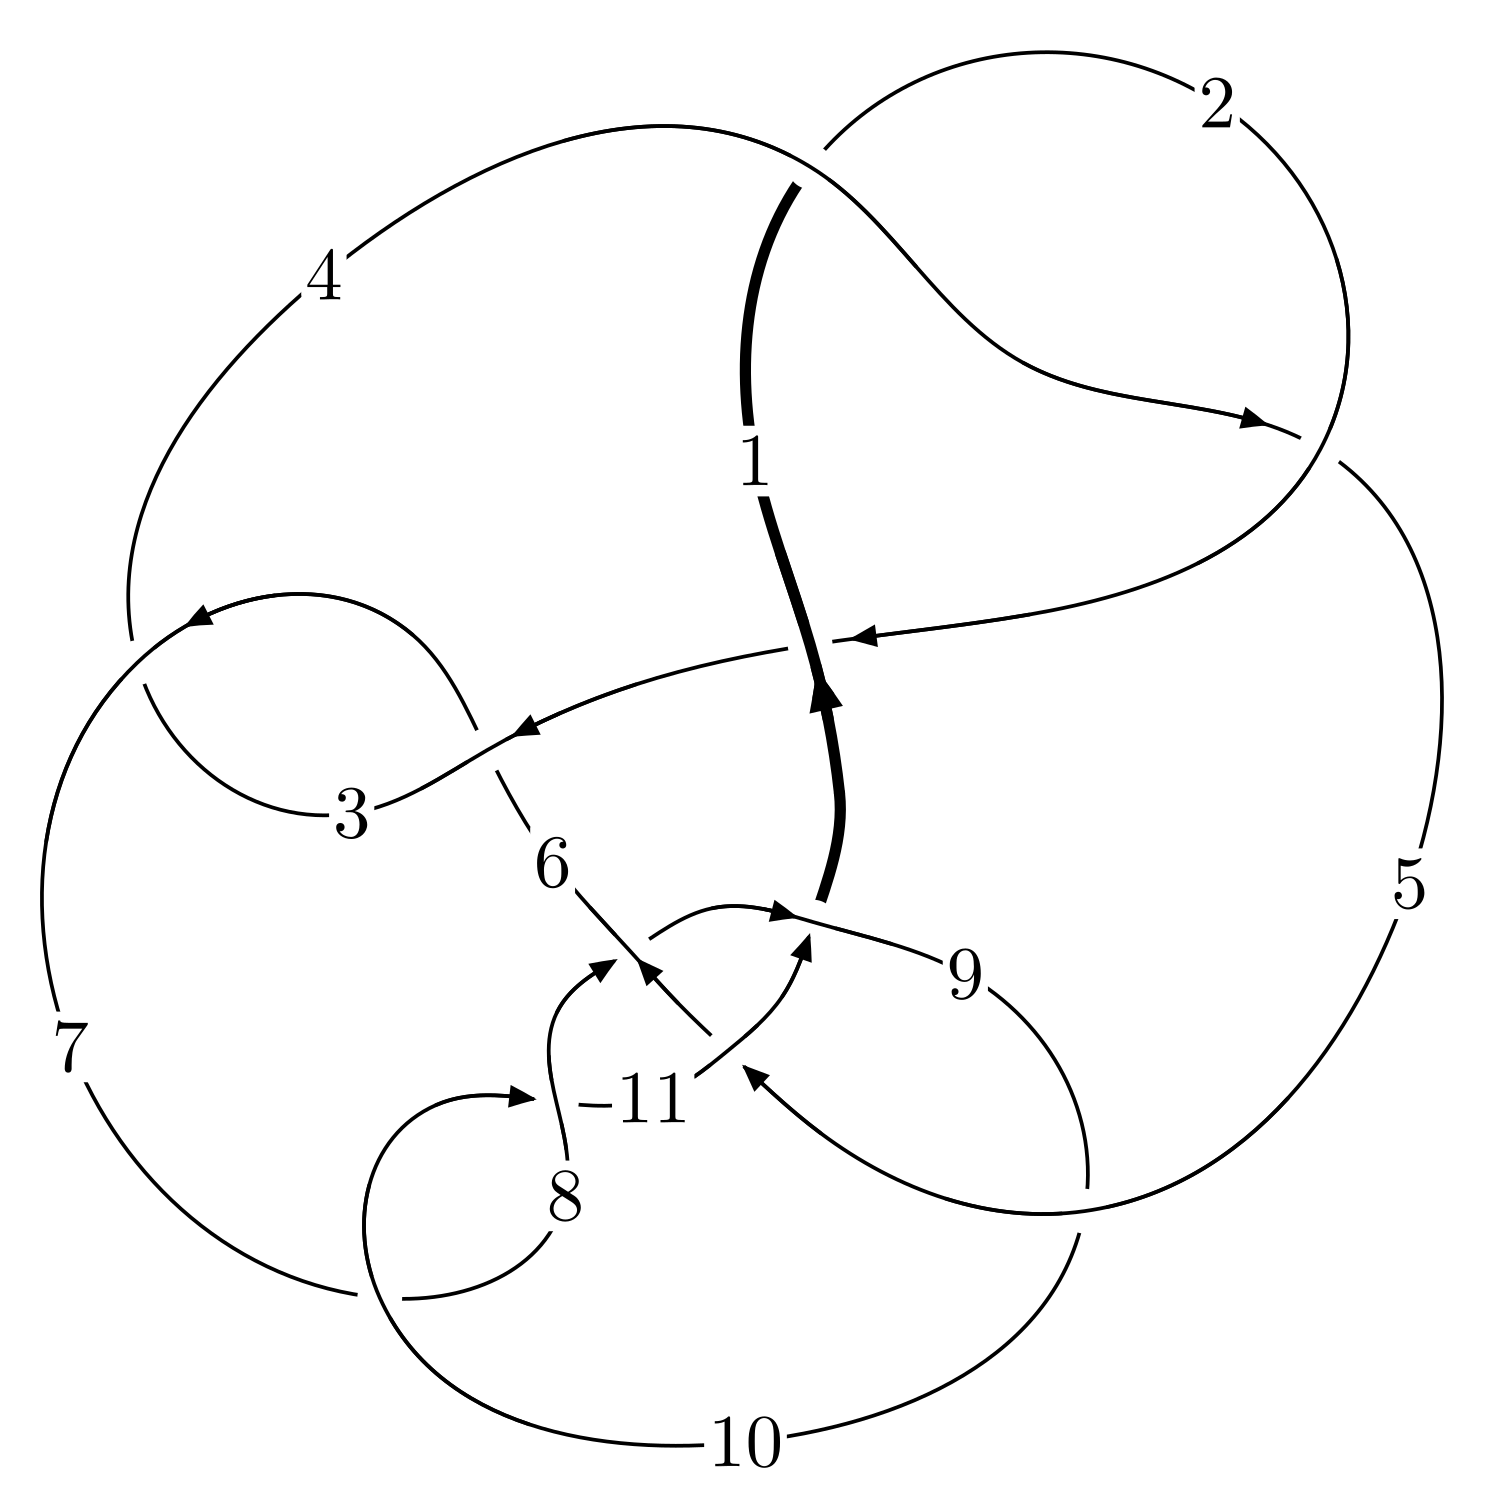
\includegraphics[width=112pt]{../../../GIT/diagram.site/Diagrams/png/273_11a_24.png}\\
\ \ \ A knot diagram\footnotemark}&
\allowdisplaybreaks
\textbf{Linearized knot diagam} \\
\cline{2-2}
 &
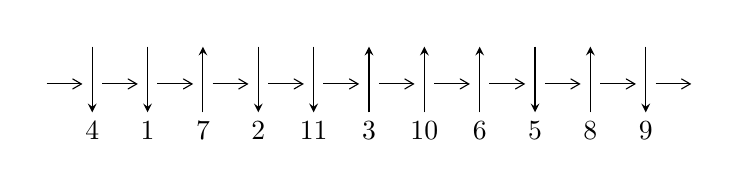
\begin{tikzpicture}[x=20pt, y=17pt]
	% nodes
	\node (C0) at (0, 0) {};
	\node (C1) at (1, 0) {};
	\node (C1U) at (1, +1) {};
	\node (C1D) at (1, -1) {4};

	\node (C2) at (2, 0) {};
	\node (C2U) at (2, +1) {};
	\node (C2D) at (2, -1) {1};

	\node (C3) at (3, 0) {};
	\node (C3U) at (3, +1) {};
	\node (C3D) at (3, -1) {7};

	\node (C4) at (4, 0) {};
	\node (C4U) at (4, +1) {};
	\node (C4D) at (4, -1) {2};

	\node (C5) at (5, 0) {};
	\node (C5U) at (5, +1) {};
	\node (C5D) at (5, -1) {11};

	\node (C6) at (6, 0) {};
	\node (C6U) at (6, +1) {};
	\node (C6D) at (6, -1) {3};

	\node (C7) at (7, 0) {};
	\node (C7U) at (7, +1) {};
	\node (C7D) at (7, -1) {10};

	\node (C8) at (8, 0) {};
	\node (C8U) at (8, +1) {};
	\node (C8D) at (8, -1) {6};

	\node (C9) at (9, 0) {};
	\node (C9U) at (9, +1) {};
	\node (C9D) at (9, -1) {5};

	\node (C10) at (10, 0) {};
	\node (C10U) at (10, +1) {};
	\node (C10D) at (10, -1) {8};

	\node (C11) at (11, 0) {};
	\node (C11U) at (11, +1) {};
	\node (C11D) at (11, -1) {9};
	\node (C12) at (12, 0) {};

	% arrows
	\draw[->,>={angle 60}]
	(C0) edge (C1) (C1) edge (C2) (C2) edge (C3) (C3) edge (C4) (C4) edge (C5) (C5) edge (C6) (C6) edge (C7) (C7) edge (C8) (C8) edge (C9) (C9) edge (C10) (C10) edge (C11) (C11) edge (C12) ;	\draw[->,>=stealth]
	(C1U) edge (C1D) (C2U) edge (C2D) (C3D) edge (C3U) (C4U) edge (C4D) (C5U) edge (C5D) (C6D) edge (C6U) (C7D) edge (C7U) (C8D) edge (C8U) (C9U) edge (C9D) (C10D) edge (C10U) (C11U) edge (C11D) ;
	\end{tikzpicture} \\
\hhline{~~} \\& 
\textbf{Solving Sequence} \\ \cline{2-2} 
 &
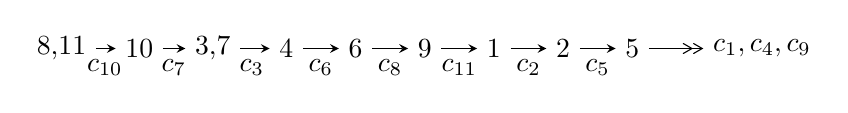
\begin{tikzpicture}[x=25pt, y=7pt]
	% node
	\node (A0) at (-1/8, 0) {8,11};
	\node (A1) at (1, 0) {10};
	\node (A2) at (33/16, 0) {3,7};
	\node (A3) at (25/8, 0) {4};
	\node (A4) at (33/8, 0) {6};
	\node (A5) at (41/8, 0) {9};
	\node (A6) at (49/8, 0) {1};
	\node (A7) at (57/8, 0) {2};
	\node (A8) at (65/8, 0) {5};
	\node (C1) at (1/2, -1) {$c_{10}$};
	\node (C2) at (3/2, -1) {$c_{7}$};
	\node (C3) at (21/8, -1) {$c_{3}$};
	\node (C4) at (29/8, -1) {$c_{6}$};
	\node (C5) at (37/8, -1) {$c_{8}$};
	\node (C6) at (45/8, -1) {$c_{11}$};
	\node (C7) at (53/8, -1) {$c_{2}$};
	\node (C8) at (61/8, -1) {$c_{5}$};
	\node (A9) at (10, 0) {$c_{1},c_{4},c_{9}$};

	% edge
	\draw[->,>=stealth]	
	(A0) edge (A1) (A1) edge (A2) (A2) edge (A3) (A3) edge (A4) (A4) edge (A5) (A5) edge (A6) (A6) edge (A7) (A7) edge (A8) ;
	\draw[->>,>={angle 60}]	
	(A8) edge (A9);
\end{tikzpicture} \\ 

\end{tabular} \\

\footnotetext{
The image of knot diagram is generated by the software ``\textbf{Draw programme}" developed by Andrew Bartholomew(\url{http://www.layer8.co.uk/maths/draw/index.htm\#Running-draw}), where we modified some parts for our purpose(\url{https://github.com/CATsTAILs/LinksPainter}).
}\phantom \\ \newline 
\centering \textbf{Ideals for irreducible components\footnotemark of $X_{\text{par}}$} 
 
\begin{align*}
I^u_{1}&=\langle 
1.30067\times10^{214} u^{83}-4.91022\times10^{214} u^{82}+\cdots+8.55509\times10^{215} b-2.17725\times10^{215},\\
\phantom{I^u_{1}}&\phantom{= \langle  }8.45896\times10^{215} u^{83}+3.25448\times10^{216} u^{82}+\cdots+8.55509\times10^{215} a-2.49116\times10^{216},\;u^{84}+2 u^{83}+\cdots+14 u+1\rangle \\
I^u_{2}&=\langle 
u^3+u^2+b-1,\;- u^5- u^4+u^2+a+u+1,\;u^6+u^5- u^4-2 u^3+u+1\rangle \\
\\
\end{align*}
\raggedright * 2 irreducible components of $\dim_{\mathbb{C}}=0$, with total 90 representations.\\
\footnotetext{All coefficients of polynomials are rational numbers. But the coefficients are sometimes approximated in decimal forms when there is not enough margin.}
\newpage
\renewcommand{\arraystretch}{1}
\centering \section*{I. $I^u_{1}= \langle 1.30\times10^{214} u^{83}-4.91\times10^{214} u^{82}+\cdots+8.56\times10^{215} b-2.18\times10^{215},\;8.46\times10^{215} u^{83}+3.25\times10^{216} u^{82}+\cdots+8.56\times10^{215} a-2.49\times10^{216},\;u^{84}+2 u^{83}+\cdots+14 u+1 \rangle$}
\flushleft \textbf{(i) Arc colorings}\\
\begin{tabular}{m{7pt} m{180pt} m{7pt} m{180pt} }
\flushright $a_{8}=$&$\begin{pmatrix}0\\u\end{pmatrix}$ \\
\flushright $a_{11}=$&$\begin{pmatrix}1\\0\end{pmatrix}$ \\
\flushright $a_{10}=$&$\begin{pmatrix}1\\u^2\end{pmatrix}$ \\
\flushright $a_{3}=$&$\begin{pmatrix}-0.988763 u^{83}-3.80414 u^{82}+\cdots-6.80025 u+2.91191\\-0.0152035 u^{83}+0.0573954 u^{82}+\cdots-3.42563 u+0.254498\end{pmatrix}$ \\
\flushright $a_{7}=$&$\begin{pmatrix}- u\\- u^3+u\end{pmatrix}$ \\
\flushright $a_{4}=$&$\begin{pmatrix}-1.04577 u^{83}-4.16450 u^{82}+\cdots-4.88381 u+2.99155\\0.0467883 u^{83}+0.218798 u^{82}+\cdots-1.83625 u+0.421194\end{pmatrix}$ \\
\flushright $a_{6}=$&$\begin{pmatrix}-1.24732 u^{83}-2.76350 u^{82}+\cdots-86.8323 u-7.08081\\-0.169313 u^{83}-0.538520 u^{82}+\cdots-6.89260 u-0.832713\end{pmatrix}$ \\
\flushright $a_{9}=$&$\begin{pmatrix}-1.41797 u^{83}-4.43349 u^{82}+\cdots+16.8513 u+4.89152\\0.467127 u^{83}+0.263584 u^{82}+\cdots+3.80614 u+0.383121\end{pmatrix}$ \\
\flushright $a_{1}=$&$\begin{pmatrix}-0.407084 u^{83}-1.47948 u^{82}+\cdots-4.70101 u+1.83199\\u^3- u\end{pmatrix}$ \\
\flushright $a_{2}=$&$\begin{pmatrix}-1.94358 u^{83}-6.48012 u^{82}+\cdots-41.4182 u+1.42713\\-0.0634831 u^{83}-0.0744360 u^{82}+\cdots-5.93872 u+0.0614765\end{pmatrix}$ \\
\flushright $a_{5}=$&$\begin{pmatrix}-1.41663 u^{83}-3.30202 u^{82}+\cdots-93.7249 u-7.91353\\-0.169313 u^{83}-0.538520 u^{82}+\cdots-6.89260 u-0.832713\end{pmatrix}$\\ \flushright $a_{5}=$&$\begin{pmatrix}-1.41663 u^{83}-3.30202 u^{82}+\cdots-93.7249 u-7.91353\\-0.169313 u^{83}-0.538520 u^{82}+\cdots-6.89260 u-0.832713\end{pmatrix}$\\&\end{tabular}
\flushleft \textbf{(ii) Obstruction class $= -1$}\\~\\
\flushleft \textbf{(iii) Cusp Shapes $= 3.48179 u^{83}+6.91671 u^{82}+\cdots-1.21890 u-4.16059$}\\~\\
\newpage\renewcommand{\arraystretch}{1}
\flushleft \textbf{(iv) u-Polynomials at the component}\newline \\
\begin{tabular}{m{50pt}|m{274pt}}
Crossings & \hspace{64pt}u-Polynomials at each crossing \\
\hline $$\begin{aligned}c_{1},c_{4}\end{aligned}$$&$\begin{aligned}
&u^{84}-7 u^{83}+\cdots-3 u+1
\end{aligned}$\\
\hline $$\begin{aligned}c_{2}\end{aligned}$$&$\begin{aligned}
&u^{84}+41 u^{83}+\cdots-157 u+1
\end{aligned}$\\
\hline $$\begin{aligned}c_{3},c_{6}\end{aligned}$$&$\begin{aligned}
&u^{84}- u^{83}+\cdots-320 u+64
\end{aligned}$\\
\hline $$\begin{aligned}c_{5}\end{aligned}$$&$\begin{aligned}
&u^{84}-6 u^{83}+\cdots-2 u+1
\end{aligned}$\\
\hline $$\begin{aligned}c_{7},c_{10}\end{aligned}$$&$\begin{aligned}
&u^{84}+2 u^{83}+\cdots+14 u+1
\end{aligned}$\\
\hline $$\begin{aligned}c_{8}\end{aligned}$$&$\begin{aligned}
&u^{84}+6 u^{83}+\cdots-1166 u-101
\end{aligned}$\\
\hline $$\begin{aligned}c_{9}\end{aligned}$$&$\begin{aligned}
&u^{84}+2 u^{83}+\cdots-418 u+367
\end{aligned}$\\
\hline $$\begin{aligned}c_{11}\end{aligned}$$&$\begin{aligned}
&u^{84}-14 u^{83}+\cdots-2 u+1
\end{aligned}$\\
\hline
\end{tabular}\\~\\
\newpage\renewcommand{\arraystretch}{1}
\flushleft \textbf{(v) Riley Polynomials at the component}\newline \\
\begin{tabular}{m{50pt}|m{274pt}}
Crossings & \hspace{64pt}Riley Polynomials at each crossing \\
\hline $$\begin{aligned}c_{1},c_{4}\end{aligned}$$&$\begin{aligned}
&y^{84}-41 y^{83}+\cdots+157 y+1
\end{aligned}$\\
\hline $$\begin{aligned}c_{2}\end{aligned}$$&$\begin{aligned}
&y^{84}+11 y^{83}+\cdots-14895 y+1
\end{aligned}$\\
\hline $$\begin{aligned}c_{3},c_{6}\end{aligned}$$&$\begin{aligned}
&y^{84}-39 y^{83}+\cdots-61440 y+4096
\end{aligned}$\\
\hline $$\begin{aligned}c_{5}\end{aligned}$$&$\begin{aligned}
&y^{84}+14 y^{83}+\cdots+6 y+1
\end{aligned}$\\
\hline $$\begin{aligned}c_{7},c_{10}\end{aligned}$$&$\begin{aligned}
&y^{84}-54 y^{83}+\cdots-14 y+1
\end{aligned}$\\
\hline $$\begin{aligned}c_{8}\end{aligned}$$&$\begin{aligned}
&y^{84}-82 y^{83}+\cdots-878594 y+10201
\end{aligned}$\\
\hline $$\begin{aligned}c_{9}\end{aligned}$$&$\begin{aligned}
&y^{84}-66 y^{83}+\cdots+5678926 y+134689
\end{aligned}$\\
\hline $$\begin{aligned}c_{11}\end{aligned}$$&$\begin{aligned}
&y^{84}-6 y^{83}+\cdots-14 y+1
\end{aligned}$\\
\hline
\end{tabular}\\~\\
\newpage\flushleft \textbf{(vi) Complex Volumes and Cusp Shapes}
$$\begin{array}{c|c|c}  
\text{Solutions to }I^u_{1}& \I (\text{vol} + \sqrt{-1}CS) & \text{Cusp shape}\\
 \hline 
\begin{aligned}
u &= \phantom{-}0.997274 + 0.064037 I \\
a &= -1.81059 - 1.67983 I \\
b &= -0.108509 + 0.553528 I\end{aligned}
 & -0.170119 + 1.192110 I & \phantom{-0.000000 } 0 \\ \hline\begin{aligned}
u &= \phantom{-}0.997274 - 0.064037 I \\
a &= -1.81059 + 1.67983 I \\
b &= -0.108509 - 0.553528 I\end{aligned}
 & -0.170119 - 1.192110 I & \phantom{-0.000000 } 0 \\ \hline\begin{aligned}
u &= -0.102288 + 0.984625 I \\
a &= -0.16025 - 1.96694 I \\
b &= \phantom{-}0.29383 + 3.01137 I\end{aligned}
 & -3.75795 + 2.95090 I & \phantom{-0.000000 } 0 \\ \hline\begin{aligned}
u &= -0.102288 - 0.984625 I \\
a &= -0.16025 + 1.96694 I \\
b &= \phantom{-}0.29383 - 3.01137 I\end{aligned}
 & -3.75795 - 2.95090 I & \phantom{-0.000000 } 0 \\ \hline\begin{aligned}
u &= -0.664606 + 0.732185 I \\
a &= -0.123840 + 0.343728 I \\
b &= \phantom{-}0.763633 + 0.462053 I\end{aligned}
 & -3.09506 + 1.90596 I & \phantom{-0.000000 } 0 \\ \hline\begin{aligned}
u &= -0.664606 - 0.732185 I \\
a &= -0.123840 - 0.343728 I \\
b &= \phantom{-}0.763633 - 0.462053 I\end{aligned}
 & -3.09506 - 1.90596 I & \phantom{-0.000000 } 0 \\ \hline\begin{aligned}
u &= -0.863087 + 0.537497 I \\
a &= \phantom{-}0.371639 - 0.064568 I \\
b &= \phantom{-}0.655881 - 0.397465 I\end{aligned}
 & -2.46714 - 6.77503 I & \phantom{-0.000000 } 0 \\ \hline\begin{aligned}
u &= -0.863087 - 0.537497 I \\
a &= \phantom{-}0.371639 + 0.064568 I \\
b &= \phantom{-}0.655881 + 0.397465 I\end{aligned}
 & -2.46714 + 6.77503 I & \phantom{-0.000000 } 0 \\ \hline\begin{aligned}
u &= -0.949424 + 0.157182 I \\
a &= -0.074074 + 0.452890 I \\
b &= \phantom{-}0.331741 + 1.326920 I\end{aligned}
 & -0.71473 - 2.85212 I & \phantom{-0.000000 } 0 \\ \hline\begin{aligned}
u &= -0.949424 - 0.157182 I \\
a &= -0.074074 - 0.452890 I \\
b &= \phantom{-}0.331741 - 1.326920 I\end{aligned}
 & -0.71473 + 2.85212 I & \phantom{-0.000000 } 0\\
 \hline 
 \end{array}$$\newpage$$\begin{array}{c|c|c}  
\text{Solutions to }I^u_{1}& \I (\text{vol} + \sqrt{-1}CS) & \text{Cusp shape}\\
 \hline 
\begin{aligned}
u &= \phantom{-}1.016320 + 0.211690 I \\
a &= \phantom{-}0.675398 + 0.703466 I \\
b &= -0.047691 + 0.460046 I\end{aligned}
 & \phantom{-}1.89935 + 0.79593 I & \phantom{-0.000000 } 0 \\ \hline\begin{aligned}
u &= \phantom{-}1.016320 - 0.211690 I \\
a &= \phantom{-}0.675398 - 0.703466 I \\
b &= -0.047691 - 0.460046 I\end{aligned}
 & \phantom{-}1.89935 - 0.79593 I & \phantom{-0.000000 } 0 \\ \hline\begin{aligned}
u &= -1.018820 + 0.211435 I \\
a &= -0.112800 + 0.423033 I \\
b &= -0.549106 + 0.960886 I\end{aligned}
 & \phantom{-}1.52052 - 3.66155 I & \phantom{-0.000000 } 0 \\ \hline\begin{aligned}
u &= -1.018820 - 0.211435 I \\
a &= -0.112800 - 0.423033 I \\
b &= -0.549106 - 0.960886 I\end{aligned}
 & \phantom{-}1.52052 + 3.66155 I & \phantom{-0.000000 } 0 \\ \hline\begin{aligned}
u &= -0.059119 + 1.083010 I \\
a &= \phantom{-}0.054493 - 0.690871 I \\
b &= -1.11124 + 1.07233 I\end{aligned}
 & -3.10217 + 5.44544 I & \phantom{-0.000000 } 0 \\ \hline\begin{aligned}
u &= -0.059119 - 1.083010 I \\
a &= \phantom{-}0.054493 + 0.690871 I \\
b &= -1.11124 - 1.07233 I\end{aligned}
 & -3.10217 - 5.44544 I & \phantom{-0.000000 } 0 \\ \hline\begin{aligned}
u &= \phantom{-}1.082570 + 0.076456 I \\
a &= -3.41552 + 1.14018 I \\
b &= \phantom{-}0.248058 - 0.161656 I\end{aligned}
 & \phantom{-}3.90317 + 1.17062 I & \phantom{-0.000000 } 0 \\ \hline\begin{aligned}
u &= \phantom{-}1.082570 - 0.076456 I \\
a &= -3.41552 - 1.14018 I \\
b &= \phantom{-}0.248058 + 0.161656 I\end{aligned}
 & \phantom{-}3.90317 - 1.17062 I & \phantom{-0.000000 } 0 \\ \hline\begin{aligned}
u &= \phantom{-}0.911327 + 0.012256 I \\
a &= \phantom{-}2.26398 - 4.32538 I \\
b &= -0.798363 + 0.238635 I\end{aligned}
 & -0.506438 - 0.641182 I & \phantom{-}14.9092 + 0. I\phantom{ +0.000000I} \\ \hline\begin{aligned}
u &= \phantom{-}0.911327 - 0.012256 I \\
a &= \phantom{-}2.26398 + 4.32538 I \\
b &= -0.798363 - 0.238635 I\end{aligned}
 & -0.506438 + 0.641182 I & \phantom{-}14.9092 + 0. I\phantom{ +0.000000I}\\
 \hline 
 \end{array}$$\newpage$$\begin{array}{c|c|c}  
\text{Solutions to }I^u_{1}& \I (\text{vol} + \sqrt{-1}CS) & \text{Cusp shape}\\
 \hline 
\begin{aligned}
u &= \phantom{-}1.079110 + 0.152121 I \\
a &= \phantom{-}2.69645 - 1.48029 I \\
b &= -0.222009 + 0.307833 I\end{aligned}
 & \phantom{-}2.03656 + 6.17754 I & \phantom{-0.000000 } 0 \\ \hline\begin{aligned}
u &= \phantom{-}1.079110 - 0.152121 I \\
a &= \phantom{-}2.69645 + 1.48029 I \\
b &= -0.222009 - 0.307833 I\end{aligned}
 & \phantom{-}2.03656 - 6.17754 I & \phantom{-0.000000 } 0 \\ \hline\begin{aligned}
u &= \phantom{-}0.453075 + 0.998389 I \\
a &= -0.39643 + 1.40161 I \\
b &= -0.93881 - 1.91477 I\end{aligned}
 & \phantom{-}3.23379 + 3.44018 I & \phantom{-0.000000 } 0 \\ \hline\begin{aligned}
u &= \phantom{-}0.453075 - 0.998389 I \\
a &= -0.39643 - 1.40161 I \\
b &= -0.93881 + 1.91477 I\end{aligned}
 & \phantom{-}3.23379 - 3.44018 I & \phantom{-0.000000 } 0 \\ \hline\begin{aligned}
u &= -0.437239 + 1.006900 I \\
a &= \phantom{-}0.042406 - 0.448835 I \\
b &= -1.137930 + 0.255603 I\end{aligned}
 & -3.77732 - 0.83071 I & \phantom{-0.000000 } 0 \\ \hline\begin{aligned}
u &= -0.437239 - 1.006900 I \\
a &= \phantom{-}0.042406 + 0.448835 I \\
b &= -1.137930 - 0.255603 I\end{aligned}
 & -3.77732 + 0.83071 I & \phantom{-0.000000 } 0 \\ \hline\begin{aligned}
u &= -1.102510 + 0.205014 I \\
a &= \phantom{-}1.050110 + 0.276781 I \\
b &= -0.982351 - 0.112643 I\end{aligned}
 & \phantom{-}4.58405 - 3.81524 I & \phantom{-0.000000 } 0 \\ \hline\begin{aligned}
u &= -1.102510 - 0.205014 I \\
a &= \phantom{-}1.050110 - 0.276781 I \\
b &= -0.982351 + 0.112643 I\end{aligned}
 & \phantom{-}4.58405 + 3.81524 I & \phantom{-0.000000 } 0 \\ \hline\begin{aligned}
u &= -0.869525 + 0.090739 I \\
a &= -0.215754 + 1.105480 I \\
b &= \phantom{-}1.26313 + 0.82270 I\end{aligned}
 & -1.87887 - 1.58264 I & -12.5915 + 7.5531 I \\ \hline\begin{aligned}
u &= -0.869525 - 0.090739 I \\
a &= -0.215754 - 1.105480 I \\
b &= \phantom{-}1.26313 - 0.82270 I\end{aligned}
 & -1.87887 + 1.58264 I & -12.5915 - 7.5531 I\\
 \hline 
 \end{array}$$\newpage$$\begin{array}{c|c|c}  
\text{Solutions to }I^u_{1}& \I (\text{vol} + \sqrt{-1}CS) & \text{Cusp shape}\\
 \hline 
\begin{aligned}
u &= -1.116610 + 0.326840 I \\
a &= -1.124930 - 0.288206 I \\
b &= \phantom{-}0.860409 + 0.470013 I\end{aligned}
 & \phantom{-}2.02563 - 9.85203 I & \phantom{-0.000000 } 0 \\ \hline\begin{aligned}
u &= -1.116610 - 0.326840 I \\
a &= -1.124930 + 0.288206 I \\
b &= \phantom{-}0.860409 - 0.470013 I\end{aligned}
 & \phantom{-}2.02563 + 9.85203 I & \phantom{-0.000000 } 0 \\ \hline\begin{aligned}
u &= -0.825783\phantom{ +0.000000I} \\
a &= -0.898341\phantom{ +0.000000I} \\
b &= \phantom{-}1.69707\phantom{ +0.000000I}\end{aligned}
 & -2.21927\phantom{ +0.000000I} & -13.1200\phantom{ +0.000000I} \\ \hline\begin{aligned}
u &= \phantom{-}0.019790 + 1.184810 I \\
a &= \phantom{-}0.09744 + 1.58758 I \\
b &= -0.74986 - 2.86475 I\end{aligned}
 & \phantom{-}1.35757 + 6.09736 I & \phantom{-0.000000 } 0 \\ \hline\begin{aligned}
u &= \phantom{-}0.019790 - 1.184810 I \\
a &= \phantom{-}0.09744 - 1.58758 I \\
b &= -0.74986 + 2.86475 I\end{aligned}
 & \phantom{-}1.35757 - 6.09736 I & \phantom{-0.000000 } 0 \\ \hline\begin{aligned}
u &= \phantom{-}0.760656 + 0.267559 I \\
a &= -1.60985 - 0.17899 I \\
b &= -0.171440 + 0.438489 I\end{aligned}
 & \phantom{-}1.30476 - 4.74367 I & \phantom{-}0.87707 + 10.18383 I \\ \hline\begin{aligned}
u &= \phantom{-}0.760656 - 0.267559 I \\
a &= -1.60985 + 0.17899 I \\
b &= -0.171440 - 0.438489 I\end{aligned}
 & \phantom{-}1.30476 + 4.74367 I & \phantom{-}0.87707 - 10.18383 I \\ \hline\begin{aligned}
u &= \phantom{-}0.753131 + 0.965934 I \\
a &= \phantom{-}0.474949 - 1.156420 I \\
b &= \phantom{-}1.32505 + 1.38024 I\end{aligned}
 & \phantom{-}2.30506 - 1.39249 I & \phantom{-0.000000 } 0 \\ \hline\begin{aligned}
u &= \phantom{-}0.753131 - 0.965934 I \\
a &= \phantom{-}0.474949 + 1.156420 I \\
b &= \phantom{-}1.32505 - 1.38024 I\end{aligned}
 & \phantom{-}2.30506 + 1.39249 I & \phantom{-0.000000 } 0 \\ \hline\begin{aligned}
u &= -0.058016 + 0.768540 I \\
a &= \phantom{-}0.315104 + 0.734938 I \\
b &= \phantom{-}0.518190 - 0.960123 I\end{aligned}
 & -1.24805 + 1.52698 I & -2.33035 - 1.80956 I\\
 \hline 
 \end{array}$$\newpage$$\begin{array}{c|c|c}  
\text{Solutions to }I^u_{1}& \I (\text{vol} + \sqrt{-1}CS) & \text{Cusp shape}\\
 \hline 
\begin{aligned}
u &= -0.058016 - 0.768540 I \\
a &= \phantom{-}0.315104 - 0.734938 I \\
b &= \phantom{-}0.518190 + 0.960123 I\end{aligned}
 & -1.24805 - 1.52698 I & -2.33035 + 1.80956 I \\ \hline\begin{aligned}
u &= -0.068869 + 1.265220 I \\
a &= -0.22787 - 1.51980 I \\
b &= \phantom{-}0.81020 + 3.04589 I\end{aligned}
 & -1.04730 + 11.43990 I & \phantom{-0.000000 } 0 \\ \hline\begin{aligned}
u &= -0.068869 - 1.265220 I \\
a &= -0.22787 + 1.51980 I \\
b &= \phantom{-}0.81020 - 3.04589 I\end{aligned}
 & -1.04730 - 11.43990 I & \phantom{-0.000000 } 0 \\ \hline\begin{aligned}
u &= \phantom{-}1.185150 + 0.478372 I \\
a &= -2.83251 + 0.12958 I \\
b &= -0.11437 - 3.23192 I\end{aligned}
 & \phantom{-}0.55551 + 1.40163 I & \phantom{-0.000000 } 0 \\ \hline\begin{aligned}
u &= \phantom{-}1.185150 - 0.478372 I \\
a &= -2.83251 - 0.12958 I \\
b &= -0.11437 + 3.23192 I\end{aligned}
 & \phantom{-}0.55551 - 1.40163 I & \phantom{-0.000000 } 0 \\ \hline\begin{aligned}
u &= -1.120340 + 0.633983 I \\
a &= -0.107831 - 0.145857 I \\
b &= -0.478833 - 0.286891 I\end{aligned}
 & -1.61526 - 4.99229 I & \phantom{-0.000000 } 0 \\ \hline\begin{aligned}
u &= -1.120340 - 0.633983 I \\
a &= -0.107831 + 0.145857 I \\
b &= -0.478833 + 0.286891 I\end{aligned}
 & -1.61526 + 4.99229 I & \phantom{-0.000000 } 0 \\ \hline\begin{aligned}
u &= -1.313920 + 0.221045 I \\
a &= \phantom{-}1.40367 - 0.49380 I \\
b &= -0.39515 - 1.46173 I\end{aligned}
 & \phantom{-}8.69358 - 1.42500 I & \phantom{-0.000000 } 0 \\ \hline\begin{aligned}
u &= -1.313920 - 0.221045 I \\
a &= \phantom{-}1.40367 + 0.49380 I \\
b &= -0.39515 + 1.46173 I\end{aligned}
 & \phantom{-}8.69358 + 1.42500 I & \phantom{-0.000000 } 0 \\ \hline\begin{aligned}
u &= -1.269980 + 0.456591 I \\
a &= \phantom{-}0.019552 + 0.257799 I \\
b &= \phantom{-}0.197110 + 0.903459 I\end{aligned}
 & \phantom{-}2.49717 - 6.15202 I & \phantom{-0.000000 } 0\\
 \hline 
 \end{array}$$\newpage$$\begin{array}{c|c|c}  
\text{Solutions to }I^u_{1}& \I (\text{vol} + \sqrt{-1}CS) & \text{Cusp shape}\\
 \hline 
\begin{aligned}
u &= -1.269980 - 0.456591 I \\
a &= \phantom{-}0.019552 - 0.257799 I \\
b &= \phantom{-}0.197110 - 0.903459 I\end{aligned}
 & \phantom{-}2.49717 + 6.15202 I & \phantom{-0.000000 } 0 \\ \hline\begin{aligned}
u &= -1.287330 + 0.518358 I \\
a &= \phantom{-}2.19968 + 0.03083 I \\
b &= \phantom{-}0.07851 - 2.92753 I\end{aligned}
 & -0.05021 - 8.32055 I & \phantom{-0.000000 } 0 \\ \hline\begin{aligned}
u &= -1.287330 - 0.518358 I \\
a &= \phantom{-}2.19968 - 0.03083 I \\
b &= \phantom{-}0.07851 + 2.92753 I\end{aligned}
 & -0.05021 + 8.32055 I & \phantom{-0.000000 } 0 \\ \hline\begin{aligned}
u &= -1.359920 + 0.328154 I \\
a &= -1.59384 + 0.34412 I \\
b &= \phantom{-}0.13897 + 1.87600 I\end{aligned}
 & \phantom{-}8.89963 - 7.63957 I & \phantom{-0.000000 } 0 \\ \hline\begin{aligned}
u &= -1.359920 - 0.328154 I \\
a &= -1.59384 - 0.34412 I \\
b &= \phantom{-}0.13897 - 1.87600 I\end{aligned}
 & \phantom{-}8.89963 + 7.63957 I & \phantom{-0.000000 } 0 \\ \hline\begin{aligned}
u &= \phantom{-}1.372270 + 0.321304 I \\
a &= -0.513421 + 1.100380 I \\
b &= -1.12473 + 0.93046 I\end{aligned}
 & \phantom{-}2.02169 - 0.07920 I & \phantom{-0.000000 } 0 \\ \hline\begin{aligned}
u &= \phantom{-}1.372270 - 0.321304 I \\
a &= -0.513421 - 1.100380 I \\
b &= -1.12473 - 0.93046 I\end{aligned}
 & \phantom{-}2.02169 + 0.07920 I & \phantom{-0.000000 } 0 \\ \hline\begin{aligned}
u &= \phantom{-}1.27275 + 0.62263 I \\
a &= \phantom{-}0.488260 - 0.932888 I \\
b &= \phantom{-}1.53439 - 0.11482 I\end{aligned}
 & \phantom{-}1.46677 + 3.41872 I & \phantom{-0.000000 } 0 \\ \hline\begin{aligned}
u &= \phantom{-}1.27275 - 0.62263 I \\
a &= \phantom{-}0.488260 + 0.932888 I \\
b &= \phantom{-}1.53439 + 0.11482 I\end{aligned}
 & \phantom{-}1.46677 - 3.41872 I & \phantom{-0.000000 } 0 \\ \hline\begin{aligned}
u &= -1.32371 + 0.54168 I \\
a &= -0.055111 - 0.254827 I \\
b &= -0.432725 - 0.905285 I\end{aligned}
 & \phantom{-}0.85835 - 11.16100 I & \phantom{-0.000000 } 0\\
 \hline 
 \end{array}$$\newpage$$\begin{array}{c|c|c}  
\text{Solutions to }I^u_{1}& \I (\text{vol} + \sqrt{-1}CS) & \text{Cusp shape}\\
 \hline 
\begin{aligned}
u &= -1.32371 - 0.54168 I \\
a &= -0.055111 + 0.254827 I \\
b &= -0.432725 + 0.905285 I\end{aligned}
 & \phantom{-}0.85835 + 11.16100 I & \phantom{-0.000000 } 0 \\ \hline\begin{aligned}
u &= \phantom{-}0.533566 + 0.191258 I \\
a &= \phantom{-}2.11026 - 0.02097 I \\
b &= \phantom{-}0.015738 - 0.400573 I\end{aligned}
 & \phantom{-}2.75270 - 0.12135 I & \phantom{-}4.31662 + 2.02203 I \\ \hline\begin{aligned}
u &= \phantom{-}0.533566 - 0.191258 I \\
a &= \phantom{-}2.11026 + 0.02097 I \\
b &= \phantom{-}0.015738 + 0.400573 I\end{aligned}
 & \phantom{-}2.75270 + 0.12135 I & \phantom{-}4.31662 - 2.02203 I \\ \hline\begin{aligned}
u &= -1.37591 + 0.55145 I \\
a &= -1.85420 - 0.20688 I \\
b &= -0.46756 + 2.62832 I\end{aligned}
 & \phantom{-}5.73608 - 12.12140 I & \phantom{-0.000000 } 0 \\ \hline\begin{aligned}
u &= -1.37591 - 0.55145 I \\
a &= -1.85420 + 0.20688 I \\
b &= -0.46756 - 2.62832 I\end{aligned}
 & \phantom{-}5.73608 + 12.12140 I & \phantom{-0.000000 } 0 \\ \hline\begin{aligned}
u &= -1.37982 + 0.60344 I \\
a &= \phantom{-}1.81821 + 0.36696 I \\
b &= \phantom{-}0.65074 - 2.69787 I\end{aligned}
 & \phantom{-}3.1034 - 17.9006 I & \phantom{-0.000000 } 0 \\ \hline\begin{aligned}
u &= -1.37982 - 0.60344 I \\
a &= \phantom{-}1.81821 - 0.36696 I \\
b &= \phantom{-}0.65074 + 2.69787 I\end{aligned}
 & \phantom{-}3.1034 + 17.9006 I & \phantom{-0.000000 } 0 \\ \hline\begin{aligned}
u &= -0.133149 + 0.453460 I \\
a &= -0.79716 + 2.36462 I \\
b &= \phantom{-}0.538862 - 0.115588 I\end{aligned}
 & -0.73011 + 6.65250 I & -2.66432 - 3.51460 I \\ \hline\begin{aligned}
u &= -0.133149 - 0.453460 I \\
a &= -0.79716 - 2.36462 I \\
b &= \phantom{-}0.538862 + 0.115588 I\end{aligned}
 & -0.73011 - 6.65250 I & -2.66432 + 3.51460 I \\ \hline\begin{aligned}
u &= \phantom{-}1.41107 + 0.70362 I \\
a &= \phantom{-}1.64088 - 0.08554 I \\
b &= \phantom{-}0.22225 + 3.33896 I\end{aligned}
 & \phantom{-}5.99281 + 3.52843 I & \phantom{-0.000000 } 0\\
 \hline 
 \end{array}$$\newpage$$\begin{array}{c|c|c}  
\text{Solutions to }I^u_{1}& \I (\text{vol} + \sqrt{-1}CS) & \text{Cusp shape}\\
 \hline 
\begin{aligned}
u &= \phantom{-}1.41107 - 0.70362 I \\
a &= \phantom{-}1.64088 + 0.08554 I \\
b &= \phantom{-}0.22225 - 3.33896 I\end{aligned}
 & \phantom{-}5.99281 - 3.52843 I & \phantom{-0.000000 } 0 \\ \hline\begin{aligned}
u &= \phantom{-}1.36356 + 0.82563 I \\
a &= -1.50074 + 0.27918 I \\
b &= -0.07330 - 3.39650 I\end{aligned}
 & \phantom{-}4.05037 + 8.85752 I & \phantom{-0.000000 } 0 \\ \hline\begin{aligned}
u &= \phantom{-}1.36356 - 0.82563 I \\
a &= -1.50074 - 0.27918 I \\
b &= -0.07330 + 3.39650 I\end{aligned}
 & \phantom{-}4.05037 - 8.85752 I & \phantom{-0.000000 } 0 \\ \hline\begin{aligned}
u &= \phantom{-}1.58214 + 0.40524 I \\
a &= \phantom{-}1.51705 + 0.56885 I \\
b &= \phantom{-}0.64537 + 3.02218 I\end{aligned}
 & \phantom{-}6.53306 + 0.44104 I & \phantom{-0.000000 } 0 \\ \hline\begin{aligned}
u &= \phantom{-}1.58214 - 0.40524 I \\
a &= \phantom{-}1.51705 - 0.56885 I \\
b &= \phantom{-}0.64537 - 3.02218 I\end{aligned}
 & \phantom{-}6.53306 - 0.44104 I & \phantom{-0.000000 } 0 \\ \hline\begin{aligned}
u &= \phantom{-}0.049986 + 0.360419 I \\
a &= \phantom{-}1.69770 + 1.17273 I \\
b &= -0.038801 - 0.987614 I\end{aligned}
 & -0.95967 + 1.37657 I & -3.31883 - 4.67522 I \\ \hline\begin{aligned}
u &= \phantom{-}0.049986 - 0.360419 I \\
a &= \phantom{-}1.69770 - 1.17273 I \\
b &= -0.038801 + 0.987614 I\end{aligned}
 & -0.95967 - 1.37657 I & -3.31883 + 4.67522 I \\ \hline\begin{aligned}
u &= \phantom{-}1.66970 + 0.27894 I \\
a &= -1.30329 - 0.71487 I \\
b &= -0.93162 - 2.84030 I\end{aligned}
 & \phantom{-}5.01931 - 4.78307 I & \phantom{-0.000000 } 0 \\ \hline\begin{aligned}
u &= \phantom{-}1.66970 - 0.27894 I \\
a &= -1.30329 + 0.71487 I \\
b &= -0.93162 + 2.84030 I\end{aligned}
 & \phantom{-}5.01931 + 4.78307 I & \phantom{-0.000000 } 0 \\ \hline\begin{aligned}
u &= \phantom{-}0.013745 + 0.300945 I \\
a &= \phantom{-}1.91747 - 2.87096 I \\
b &= -0.416432 - 0.110948 I\end{aligned}
 & \phantom{-}1.66501 + 1.71486 I & \phantom{-}1.361742 - 0.047755 I\\
 \hline 
 \end{array}$$\newpage$$\begin{array}{c|c|c}  
\text{Solutions to }I^u_{1}& \I (\text{vol} + \sqrt{-1}CS) & \text{Cusp shape}\\
 \hline 
\begin{aligned}
u &= \phantom{-}0.013745 - 0.300945 I \\
a &= \phantom{-}1.91747 + 2.87096 I \\
b &= -0.416432 + 0.110948 I\end{aligned}
 & \phantom{-}1.66501 - 1.71486 I & \phantom{-}1.361742 + 0.047755 I \\ \hline\begin{aligned}
u &= -0.234317\phantom{ +0.000000I} \\
a &= \phantom{-}1.53674\phantom{ +0.000000I} \\
b &= \phantom{-}1.46885\phantom{ +0.000000I}\end{aligned}
 & -2.49567\phantom{ +0.000000I} & -2.13160\phantom{ +0.000000I} \\ \hline\begin{aligned}
u &= -0.122932 + 0.103046 I \\
a &= \phantom{-}5.15612 - 0.93081 I \\
b &= \phantom{-}0.615821 - 0.504298 I\end{aligned}
 & -2.25525 + 1.15492 I & -4.97585 - 0.17312 I \\ \hline\begin{aligned}
u &= -0.122932 - 0.103046 I \\
a &= \phantom{-}5.15612 + 0.93081 I \\
b &= \phantom{-}0.615821 + 0.504298 I\end{aligned}
 & -2.25525 - 1.15492 I & -4.97585 + 0.17312 I\\
 \hline 
 \end{array}$$\newpage\newpage\renewcommand{\arraystretch}{1}
\centering \section*{II. $I^u_{2}= \langle u^3+u^2+b-1,\;- u^5- u^4+u^2+a+u+1,\;u^6+u^5- u^4-2 u^3+u+1 \rangle$}
\flushleft \textbf{(i) Arc colorings}\\
\begin{tabular}{m{7pt} m{180pt} m{7pt} m{180pt} }
\flushright $a_{8}=$&$\begin{pmatrix}0\\u\end{pmatrix}$ \\
\flushright $a_{11}=$&$\begin{pmatrix}1\\0\end{pmatrix}$ \\
\flushright $a_{10}=$&$\begin{pmatrix}1\\u^2\end{pmatrix}$ \\
\flushright $a_{3}=$&$\begin{pmatrix}u^5+u^4- u^2- u-1\\- u^3- u^2+1\end{pmatrix}$ \\
\flushright $a_{7}=$&$\begin{pmatrix}- u\\- u^3+u\end{pmatrix}$ \\
\flushright $a_{4}=$&$\begin{pmatrix}u^5+u^4- u^2- u-1\\- u^3- u^2+1\end{pmatrix}$ \\
\flushright $a_{6}=$&$\begin{pmatrix}- u\\- u^3+u\end{pmatrix}$ \\
\flushright $a_{9}=$&$\begin{pmatrix}u^3\\u^5- u^3+u\end{pmatrix}$ \\
\flushright $a_{1}=$&$\begin{pmatrix}u^3\\u^3- u\end{pmatrix}$ \\
\flushright $a_{2}=$&$\begin{pmatrix}u^5+u^4+u^3- u^2- u-1\\- u^2- u+1\end{pmatrix}$ \\
\flushright $a_{5}=$&$\begin{pmatrix}- u^3\\- u^3+u\end{pmatrix}$\\ \flushright $a_{5}=$&$\begin{pmatrix}- u^3\\- u^3+u\end{pmatrix}$\\&\end{tabular}
\flushleft \textbf{(ii) Obstruction class $= 1$}\\~\\
\flushleft \textbf{(iii) Cusp Shapes $= 3 u^5- u^4+u^3+2 u^2+3 u-5$}\\~\\
\newpage\renewcommand{\arraystretch}{1}
\flushleft \textbf{(iv) u-Polynomials at the component}\newline \\
\begin{tabular}{m{50pt}|m{274pt}}
Crossings & \hspace{64pt}u-Polynomials at each crossing \\
\hline $$\begin{aligned}c_{1}\end{aligned}$$&$\begin{aligned}
&(u-1)^6
\end{aligned}$\\
\hline $$\begin{aligned}c_{2},c_{4}\end{aligned}$$&$\begin{aligned}
&(u+1)^6
\end{aligned}$\\
\hline $$\begin{aligned}c_{3},c_{6}\end{aligned}$$&$\begin{aligned}
&u^6
\end{aligned}$\\
\hline $$\begin{aligned}c_{5},c_{8}\end{aligned}$$&$\begin{aligned}
&u^6-3 u^5+5 u^4-4 u^3+2 u^2- u+1
\end{aligned}$\\
\hline $$\begin{aligned}c_{7},c_{9},c_{11}\end{aligned}$$&$\begin{aligned}
&u^6- u^5- u^4+2 u^3- u+1
\end{aligned}$\\
\hline $$\begin{aligned}c_{10}\end{aligned}$$&$\begin{aligned}
&u^6+u^5- u^4-2 u^3+u+1
\end{aligned}$\\
\hline
\end{tabular}\\~\\
\newpage\renewcommand{\arraystretch}{1}
\flushleft \textbf{(v) Riley Polynomials at the component}\newline \\
\begin{tabular}{m{50pt}|m{274pt}}
Crossings & \hspace{64pt}Riley Polynomials at each crossing \\
\hline $$\begin{aligned}c_{1},c_{2},c_{4}\end{aligned}$$&$\begin{aligned}
&(y-1)^6
\end{aligned}$\\
\hline $$\begin{aligned}c_{3},c_{6}\end{aligned}$$&$\begin{aligned}
&y^6
\end{aligned}$\\
\hline $$\begin{aligned}c_{5},c_{8}\end{aligned}$$&$\begin{aligned}
&y^6+y^5+5 y^4+6 y^2+3 y+1
\end{aligned}$\\
\hline $$\begin{aligned}c_{7},c_{9},c_{10}\\c_{11}\end{aligned}$$&$\begin{aligned}
&y^6-3 y^5+5 y^4-4 y^3+2 y^2- y+1
\end{aligned}$\\
\hline
\end{tabular}\\~\\
\newpage\flushleft \textbf{(vi) Complex Volumes and Cusp Shapes}
$$\begin{array}{c|c|c}  
\text{Solutions to }I^u_{2}& \I (\text{vol} + \sqrt{-1}CS) & \text{Cusp shape}\\
 \hline 
\begin{aligned}
u &= \phantom{-}1.002190 + 0.295542 I \\
a &= -2.25915 + 1.43225 I \\
b &= -0.66103 - 1.45708 I\end{aligned}
 & \phantom{-}0.245672 + 0.924305 I & \phantom{-}0.60470 + 5.55069 I \\ \hline\begin{aligned}
u &= \phantom{-}1.002190 - 0.295542 I \\
a &= -2.25915 - 1.43225 I \\
b &= -0.66103 + 1.45708 I\end{aligned}
 & \phantom{-}0.245672 - 0.924305 I & \phantom{-}0.60470 - 5.55069 I \\ \hline\begin{aligned}
u &= -0.428243 + 0.664531 I \\
a &= -0.655968 - 0.098281 I \\
b &= \phantom{-}0.769407 + 0.497010 I\end{aligned}
 & -3.53554 + 0.92430 I & -6.31051 - 0.25702 I \\ \hline\begin{aligned}
u &= -0.428243 - 0.664531 I \\
a &= -0.655968 + 0.098281 I \\
b &= \phantom{-}0.769407 - 0.497010 I\end{aligned}
 & -3.53554 - 0.92430 I & -6.31051 + 0.25702 I \\ \hline\begin{aligned}
u &= -1.073950 + 0.558752 I \\
a &= \phantom{-}0.415113 + 0.381252 I \\
b &= \phantom{-}0.391622 - 0.558752 I\end{aligned}
 & -1.64493 - 5.69302 I & -0.29418 + 8.33058 I \\ \hline\begin{aligned}
u &= -1.073950 - 0.558752 I \\
a &= \phantom{-}0.415113 - 0.381252 I \\
b &= \phantom{-}0.391622 + 0.558752 I\end{aligned}
 & -1.64493 + 5.69302 I & -0.29418 - 8.33058 I\\
 \hline 
 \end{array}$$\newpage
\newpage\renewcommand{\arraystretch}{1}
\centering \section*{ III. u-Polynomials}
\begin{tabular}{m{50pt}|m{274pt}}
Crossings & \hspace{64pt}u-Polynomials at each crossing \\
\hline $$\begin{aligned}c_{1}\end{aligned}$$&$\begin{aligned}
&((u-1)^6)(u^{84}-7 u^{83}+\cdots-3 u+1)
\end{aligned}$\\
\hline $$\begin{aligned}c_{2}\end{aligned}$$&$\begin{aligned}
&((u+1)^6)(u^{84}+41 u^{83}+\cdots-157 u+1)
\end{aligned}$\\
\hline $$\begin{aligned}c_{3},c_{6}\end{aligned}$$&$\begin{aligned}
&u^6(u^{84}- u^{83}+\cdots-320 u+64)
\end{aligned}$\\
\hline $$\begin{aligned}c_{4}\end{aligned}$$&$\begin{aligned}
&((u+1)^6)(u^{84}-7 u^{83}+\cdots-3 u+1)
\end{aligned}$\\
\hline $$\begin{aligned}c_{5}\end{aligned}$$&$\begin{aligned}
&(u^6-3 u^5+5 u^4-4 u^3+2 u^2- u+1)(u^{84}-6 u^{83}+\cdots-2 u+1)
\end{aligned}$\\
\hline $$\begin{aligned}c_{7}\end{aligned}$$&$\begin{aligned}
&(u^6- u^5- u^4+2 u^3- u+1)(u^{84}+2 u^{83}+\cdots+14 u+1)
\end{aligned}$\\
\hline $$\begin{aligned}c_{8}\end{aligned}$$&$\begin{aligned}
&(u^6-3 u^5+5 u^4-4 u^3+2 u^2- u+1)(u^{84}+6 u^{83}+\cdots-1166 u-101)
\end{aligned}$\\
\hline $$\begin{aligned}c_{9}\end{aligned}$$&$\begin{aligned}
&(u^6- u^5- u^4+2 u^3- u+1)(u^{84}+2 u^{83}+\cdots-418 u+367)
\end{aligned}$\\
\hline $$\begin{aligned}c_{10}\end{aligned}$$&$\begin{aligned}
&(u^6+u^5- u^4-2 u^3+u+1)(u^{84}+2 u^{83}+\cdots+14 u+1)
\end{aligned}$\\
\hline $$\begin{aligned}c_{11}\end{aligned}$$&$\begin{aligned}
&(u^6- u^5- u^4+2 u^3- u+1)(u^{84}-14 u^{83}+\cdots-2 u+1)
\end{aligned}$\\
\hline
\end{tabular}\newpage\renewcommand{\arraystretch}{1}
\centering \section*{ IV. Riley Polynomials}
\begin{tabular}{m{50pt}|m{274pt}}
Crossings & \hspace{64pt}Riley Polynomials at each crossing \\
\hline $$\begin{aligned}c_{1},c_{4}\end{aligned}$$&$\begin{aligned}
&((y-1)^6)(y^{84}-41 y^{83}+\cdots+157 y+1)
\end{aligned}$\\
\hline $$\begin{aligned}c_{2}\end{aligned}$$&$\begin{aligned}
&((y-1)^6)(y^{84}+11 y^{83}+\cdots-14895 y+1)
\end{aligned}$\\
\hline $$\begin{aligned}c_{3},c_{6}\end{aligned}$$&$\begin{aligned}
&y^6(y^{84}-39 y^{83}+\cdots-61440 y+4096)
\end{aligned}$\\
\hline $$\begin{aligned}c_{5}\end{aligned}$$&$\begin{aligned}
&(y^6+y^5+5 y^4+6 y^2+3 y+1)(y^{84}+14 y^{83}+\cdots+6 y+1)
\end{aligned}$\\
\hline $$\begin{aligned}c_{7},c_{10}\end{aligned}$$&$\begin{aligned}
&(y^6-3 y^5+5 y^4-4 y^3+2 y^2- y+1)(y^{84}-54 y^{83}+\cdots-14 y+1)
\end{aligned}$\\
\hline $$\begin{aligned}c_{8}\end{aligned}$$&$\begin{aligned}
&(y^6+y^5+5 y^4+6 y^2+3 y+1)(y^{84}-82 y^{83}+\cdots-878594 y+10201)
\end{aligned}$\\
\hline $$\begin{aligned}c_{9}\end{aligned}$$&$\begin{aligned}
&(y^6-3 y^5+5 y^4-4 y^3+2 y^2- y+1)\\
&\cdot(y^{84}-66 y^{83}+\cdots+5678926 y+134689)
\end{aligned}$\\
\hline $$\begin{aligned}c_{11}\end{aligned}$$&$\begin{aligned}
&(y^6-3 y^5+5 y^4-4 y^3+2 y^2- y+1)(y^{84}-6 y^{83}+\cdots-14 y+1)
\end{aligned}$\\
\hline
\end{tabular}
\vskip 2pc
\end{document}